\chapter{WinEdt v10 and Above}
\section{}
\subsection{Options Interface}
In version 10 and above the procedure has changed.  Every thing is accessed through the \textit{Options Interface}.  Right click on the toolbar and select the button for it (see \figurename~\ref{fig:openingoptionsinterface}).  The \textit{Options Interface} is shown in \figurename~\ref{fig:optionsinterface}.
\begin{figure}
	\centering
	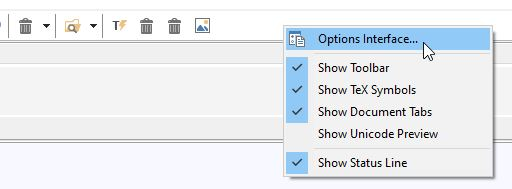
\includegraphics[width=3.25in]{openingoptionsinterface}
	\caption[Opening the \textit{Options Interface} panel]{Opening the \textit{Options Interface} panel.}
	\label{fig:openingoptionsinterface}
\end{figure}

\begin{figure}
	\centering
	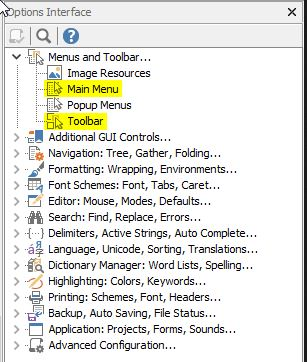
\includegraphics[width=2.25in]{optionsinterface}
	\caption[The \textit{Options Interface} panel]{The \textit{Options Interface} panel.}
	\label{fig:optionsinterface}
\end{figure}


\section{Menu Items}
\subsection{Add Custom Commands to TeX Menu}
\label{sec:addmenuitems}
\begin{numberedlist}
	\item Open the \textit{Main Menu} document from the \textit{Options Interface} panel.  This will be called \emph{File 1}.
	\item Find the section: \textcode{MENU="TeX\_Menu"}.
	\item Find the end of the \textcode{ITEM="TeXify"} menu item.  The entries will be added after this item, i.e., after the \textcode{REQ\_FILTER...} line.
	\item Open the file \textcode{.\tbs{}src V10 and Above\tbs{}MainMenu.ini} that is included in this repository.  This will be \emph{File 2}.  The contents look like the code below.
	\item Copy the contents from the \emph{File 2} into the specified location of \emph{File 1}.
	\item Save the file.
	\item Right click on the \emph{Main Menu} node in the \emph{Options Interface} and click \emph{Load Script}.
	\item Your \emph{TeX} menu should look like that in \figurename~\ref{fig:texmenu}.
\end{numberedlist}

\begin{plainlist}
	\item \textcode{ITEM="-"}
	\item \textcode{ITEM="Make\_Document"}
	\begin{plainlist}
		\item \textcode{CAPTION="Make Document"}
		\item \textcode{IMAGE="TeXTeXif"}
		\item \textcode{SAVE\_INPUT=1}
		\item \textcode{MACRO="Run('\%P\tbs{}run\_make\_document.bat ""\%N""','\%P',0,0,"}
		\begin{plainlist}
			\item \textcode{'Make Document',1,1);"}
		\end{plainlist}
		\item \textcode{REQ\_FILTER=:"\%!M=TeX"|"\%!M=TeX:STY"|"\%!M=TeX:AUX"}
	\end{plainlist}
	\item \textcode{ITEM="Clean\_Temp\_Files"}
	\begin{plainlist}
		\item \textcode{CAPTION="Delete Temporary Files"}
		\item \textcode{IMAGE="Recycle"}
		\item \textcode{SAVE\_INPUT=1}
		\item \textcode{MACRO="Run('clean\_temp\_files.bat','\%P',0,0,'Clean Temp Files',1,1);"}
	\end{plainlist}
	\item \textcode{ITEM="Clean\_All\_Output"}
	\begin{plainlist}
		\item \textcode{CAPTION="Delete All Output Files"}
		\item \textcode{IMAGE="Recycle"}
		\item \textcode{SAVE\_INPUT=1}
		\item \textcode{MACRO="Run('clean\_all\_output.bat','\%P',0,0,"}
		\begin{plainlist}
			\item \textcode{'Clean All Output Files',1,1);"}
		\end{plainlist}
	\end{plainlist}
	\item \textcode{ITEM="Convert\_All\_Images"}
	\begin{plainlist}
		\item \textcode{CAPTION="Convert All Images"}
		\item \textcode{IMAGE="Image"}
		\item \textcode{SAVE\_INPUT=1}
		\item \textcode{MACRO="Run('convert\_all\_images.bat','\%P\tbs{}Figures\tbs{}Image Sources',"}
		\begin{plainlist}
			\item \textcode{0,0,'Convert All Images',1,1);"}
		\end{plainlist}
	\end{plainlist}
\end{plainlist}

\begin{figure}
	\centering
	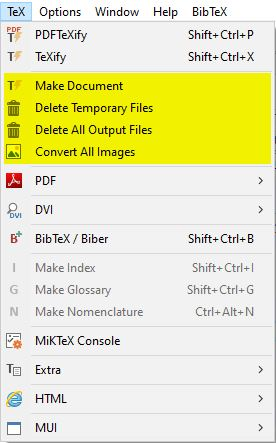
\includegraphics[width=2.25in]{texmenu}
	\caption[The \textit{TeX} menu with added items]{The \textit{TeX} menu with added items.}
	\label{fig:texmenu}
\end{figure}

\subsection{Change Shortcut Keys to Existing Commands}
Find the two menu items below and change the short cut keys to match the ones below in red.

\begin{code}[\codenumbering]{}
	\codeitemnonumber ITEM="Close"
	    \stepcodelevel{}
	    \codeitemnonumber CAPTION="\&Close"
	    \codeitemnonumber IMAGE="Close"
	    \codeitemnonumber MACRO="CloseDoc;"
	    \codeitemnonumber \warning{SHORTCUT="16471::Ctrl+W"}
	    \codeitemnonumber REQ\_DOCUMENT=1
\end{code}

\begin{code}[\codenumbering]{}
	\codeitemnonumber ITEM="\$Toggle\_Wrap/NoWrap"
		\stepcodelevel{}
	    \codeitemnonumber CAPTION="Toggle Wrap/NoWrap"
	    \codeitemnonumber MACRO="SetWrap;"
	    \codeitemnonumber \warning{SHORTCUT="16499::Ctrl+F4"}
	    \codeitemnonumber REQ\_DOCUMENT=1
\end{code}

\section{Add Toolbar Buttons}
To add toolbar buttons, start by opening the \emph{Toolbar.ini} file.  Right click on the \emph{Toolbar} node (see \figurename~\ref{fig:optionsinterface}) and select \emph{Open} or double click the node.

\subsection{Add \textit{Save All}}
Find the line:
\begin{plainlist}
	\item \textcode{BUTTON="Save"}
\end{plainlist}

and just below it add:
\begin{plainlist}
	\item \textcode{BUTTON="Save\_All"}
\end{plainlist}

\subsection{Custom Processing Buttons}
\important{For this to work, you must first add the custom menu items from \sectionname~\ref{sec:addmenuitems}.}

Go to the end of the main toolbar entry (\textcode{TOOLBAR="Toolbar\_TeX"}) and add the following lines:
\begin{plainlist}
	\item \textcode{BUTTON="|"}
	\item \textcode{BUTTON="Make\_Document"}
	\item \textcode{BUTTON="Clean\_Temp\_Files"}
	\item \textcode{BUTTON="Clean\_All\_Output"}
	\item \textcode{BUTTON="Convert\_All\_Images"}
\end{plainlist}
Save the file, right click on the \emph{Toolbar} node, and click \emph{Load Script}.

\section{Templates}
   \begin{numberedlist}
       \item Open the location: \textcode{\%b\tbs{}Templates\tbs{}LaTeX\tbs{}Figure.ltx}.  Example locations are:
       \begin{plainlist}
           \item \textcode{C:\tbs{}Users\tbs{}lance\tbs{}WinEdt Team\tbs{}WinEdt 11\tbs{}Templates\tbs{}LaTeX\tbs{}Figure.ltx}
           \item \textcode{C:\tbs{}Program Files\tbs{}WinEdt Team\tbs{}WinEdt 11\tbs{}Templates\tbs{}LaTeX\tbs{}Figure.ltx}
       \end{plainlist}
       \item Overwrite the files in that directory with the ones from:
       \begin{plainlist}
           \item \textcode{C:\tbs{}Custom Program Files\tbs{}WinEdt\tbs{}src V10 and Above\tbs{}Templates}
       \end{plainlist}
   \end{numberedlist}

\section{Running Multiple Instances}
\begin{numberedlist}
	\item Select the \textcode{Additional Preferences} section of the \textcode{Application: ...} as shown in \figurename~\ref{fig:additionalpreferences}.
	\item Change the line \textcode{RUN\_ONE\_INSTANCE\_ONLY=1} to \textcode{RUN\_ONE\_INSTANCE\_ONLY=0}.
\end{numberedlist}
\begin{figure}
	\centering
	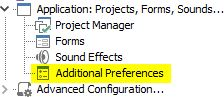
\includegraphics[width=2.5in]{additionalpreferences}
	\caption[The location of \textcode{Additional Preferences} on the \textit{Options Interface} panel]{The location of \textcode{Additional Preferences} on the \textit{Options Interface} panel.}
	\label{fig:additionalpreferences}
\end{figure}


\section{Keyboard Shortcuts}
For some keyboard shortcuts, Windows intercepts them and they do not reach \winedt{}.  This is because \winedt{} uses the MDI interface.  To remap toggling of tabs, download and install \powertoys{} (\href{https://github.com/microsoft/PowerToys}{PowerToys on Github})
\begin{outline}
	\item Add the keyboard short cut to \emph{PowerToys}.
	\begin{outline}
		\item Open \textcode{PowerToys} and go to \emph{Keyboard Manager}$\rightarrow$\emph{Remap a shortcut}
		\item Add a keyboard shortcut to remap \textcode{Ctrl+Tab} to \textcode{Shift+F2} for \winedt{}
	\end{outline}
	\item Remove the short cut from \winedt{}.
	\begin{outline}
		\item Select the \textcode{Main Menu} section of the \textcode{Menu and Toolbar...} as shown in \figurename~\ref{fig:optionsinterface}.
		\item Search for the \textcode{ITEM="Next\_MDI\_Window"} entry.
		\item Delete the \textcode{Ctrl+Tab} from the \textcode{SHORTCUT="Ctrl+Tab"} line.
	\end{outline}
\end{outline}
\begin{figure}
	\centering
	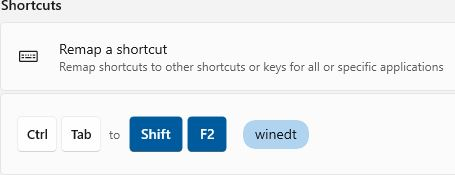
\includegraphics[width=2.5in]{powertoyssettings}
	\caption[The \powertoys{} keyboard remapping]{The \powertoys{} keyboard remapping.}
	\label{fig:powertoyssettings}
\end{figure}

\section{Tabs}
   \begin{numberedlist}
   	\item \textcode{Options$\rightarrow$Preferences$\rightarrow$Tabs}
   	\item Check \textit{Allow Keyboard Tabs}
   \end{numberedlist}

\section{User Dictionary}
\begin{numberedlist}
	\item Expand the \textit{Dictionary Manager:...} menu from the \textit{Options Interface} panel.
	\item Open the \textit{Word Lists (Dictionaries).ini} file.
	\item Find the \textcode{DICTIONARY="User (Addon)"} line.
	\item Edit the \textcode{FILE} line to point to use dictionary in the custom program files directory, e.g.:
	\begin{plainlist}
		\item \textcode{FILE="C:\tbs{}Custom Program Files\tbs{}WinEdt\tbs{}Dictionary\tbs{}User.dic"}
	\end{plainlist}
\end{numberedlist}

\section{Keywords and Syntax Highlighting}
\subsection{Fields}
\begin{numberedlist}
	\item Expand the \textit{Highlighting:...} menu from the \textit{Options Interface} panel.
	\item Open the \textit{Keywords.ini} file.
	\item Find the \textcode{KEYWORD\_GROUP="BibTeX Fields"} line.
	\item Add the items below into the list.
	\item Right click on the \textit{Keywords} node and select \textit{Load Script}.
\end{numberedlist}
\begin{plainlist}
%	\item \textcode{abstract}
%	\item \textcode{affiliation}
	\item \textcode{assignee}
	\item \textcode{day}
	\item \textcode{filedday}
	\item \textcode{filedmonth}
	\item \textcode{filedyear}
	\item \textcode{href}
	\item \textcode{id}
	\item \textcode{issuedday}
	\item \textcode{issuedmonth}
	\item \textcode{issuedyear}
	\item \textcode{logline}
	\item \textcode{pubday}
	\item \textcode{pubmonth}
	\item \textcode{pubyear}
	\item \textcode{speid}
	\item \textcode{websitename}
\end{plainlist}

\subsection{BibTeX Entry Types}
Follow the procedure similar to above, but search for the \textcode{KEYWORD\_GROUP="BibTeX"} line and add the following:
\begin{plainlist}
	\item \textcode{WEBHREF}
\end{plainlist}

\section{Paragraph and Wrapping}
\begin{numberedlist}
	\item Expand the \textit{Formatting: Wrapping...} menu from the \textit{Options Interface} panel.
	\item Open the \textit{Paragraphs} file.
	\item Find the \textcode{[PARAGRAPHS]} line.
	\item Find and edit the groups below.
	\item Right click on the \textit{Formatting: Wrapping...} node and select \textit{Load Script}.
\end{numberedlist}
\begin{code}[\codenumbering]{}
	\codeitemnonumber PARAGRAPH="	" // Tab (not a space!)
	\stepcodelevel{}
	\codeitemnonumber MODE\_FILTER="*"
	\codeitemnonumber \warning{ALLOW\_SOFT\_WRAP=1}
	\codeitemnonumber CASE\_SENSITIVE=1
	\codeitemnonumber OFFSET=1
	\codeitemnonumber \warning{OFFSET\_BY=4}
	\prevcodelevel{}
\end{code}
%  ALLOW_SOFT_WRAP=0
%  OFFSET_BY=0 